


\tikzset{every picture/.style={line width=0.75pt}} %set default line width to 0.75pt        

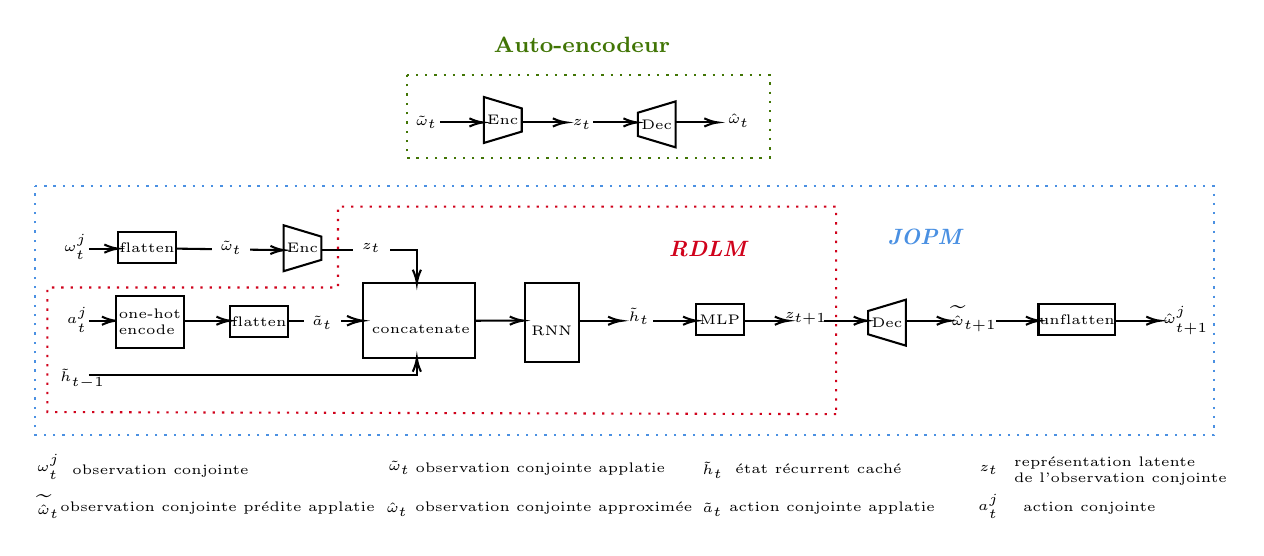
\begin{tikzpicture}[x=0.75pt,y=0.75pt,yscale=-1,xscale=1]
    %uncomment if require: \path (0,2102); %set diagram left start at 0, and has height of 2102

    %Straight Lines [id:da9858789281072494] 
    \draw    (58,1209.26) -- (70,1209.26) ;
    \draw [shift={(72,1209.26)}, rotate = 180] [color={rgb, 255:red, 0; green, 0; blue, 0 }  ][line width=0.75]    (6.56,-1.97) .. controls (4.17,-0.84) and (1.99,-0.18) .. (0,0) .. controls (1.99,0.18) and (4.17,0.84) .. (6.56,1.97)   ;
    %Straight Lines [id:da30111095973058666] 
    \draw    (58,1244) -- (68.83,1244) ;
    \draw [shift={(70.83,1244)}, rotate = 180] [color={rgb, 255:red, 0; green, 0; blue, 0 }  ][line width=0.75]    (6.56,-1.97) .. controls (4.17,-0.84) and (1.99,-0.18) .. (0,0) .. controls (1.99,0.18) and (4.17,0.84) .. (6.56,1.97)   ;
    %Straight Lines [id:da667552245584323] 
    \draw    (58,1270) -- (216,1270) -- (216,1264) ;
    \draw [shift={(216,1262)}, rotate = 90] [color={rgb, 255:red, 0; green, 0; blue, 0 }  ][line width=0.75]    (6.56,-1.97) .. controls (4.17,-0.84) and (1.99,-0.18) .. (0,0) .. controls (1.99,0.18) and (4.17,0.84) .. (6.56,1.97)   ;
    %Straight Lines [id:da474165275030325] 
    \draw    (102,1244) -- (124,1244) ;
    \draw [shift={(126,1244)}, rotate = 180] [color={rgb, 255:red, 0; green, 0; blue, 0 }  ][line width=0.75]    (6.56,-1.97) .. controls (4.17,-0.84) and (1.99,-0.18) .. (0,0) .. controls (1.99,0.18) and (4.17,0.84) .. (6.56,1.97)   ;
    %Straight Lines [id:da9904985642486432] 
    \draw    (154,1244) -- (188,1244) ;
    \draw [shift={(190,1244)}, rotate = 180] [color={rgb, 255:red, 0; green, 0; blue, 0 }  ][line width=0.75]    (7.65,-2.3) .. controls (4.86,-0.97) and (2.31,-0.21) .. (0,0) .. controls (2.31,0.21) and (4.86,0.98) .. (7.65,2.3)   ;
    %Straight Lines [id:da030414880825802904] 
    \draw    (100,1209.26) -- (150,1209.97) ;
    \draw [shift={(152,1210)}, rotate = 180.81] [color={rgb, 255:red, 0; green, 0; blue, 0 }  ][line width=0.75]    (6.56,-1.97) .. controls (4.17,-0.84) and (1.99,-0.18) .. (0,0) .. controls (1.99,0.18) and (4.17,0.84) .. (6.56,1.97)   ;
    %Shape: Trapezoid [id:dp21506927038478751] 
    \draw   (151.77,1198) -- (170,1203.47) -- (170,1214.68) -- (151.77,1220.14) -- cycle ;
    %Straight Lines [id:da5495855493758877] 
    \draw    (170,1210) -- (216,1210) -- (216,1224) ;
    \draw [shift={(216,1226)}, rotate = 270] [color={rgb, 255:red, 0; green, 0; blue, 0 }  ][line width=0.75]    (6.56,-1.97) .. controls (4.17,-0.84) and (1.99,-0.18) .. (0,0) .. controls (1.99,0.18) and (4.17,0.84) .. (6.56,1.97)   ;
    %Straight Lines [id:da9334314266641691] 
    \draw    (244,1244) -- (265.33,1243.94) ;
    \draw [shift={(267.33,1243.94)}, rotate = 179.85] [color={rgb, 255:red, 0; green, 0; blue, 0 }  ][line width=0.75]    (6.56,-1.97) .. controls (4.17,-0.84) and (1.99,-0.18) .. (0,0) .. controls (1.99,0.18) and (4.17,0.84) .. (6.56,1.97)   ;
    %Straight Lines [id:da6494490821033114] 
    \draw    (293.89,1244.03) -- (312.72,1244.03) ;
    \draw [shift={(314.72,1244.03)}, rotate = 180] [color={rgb, 255:red, 0; green, 0; blue, 0 }  ][line width=0.75]    (6.56,-1.97) .. controls (4.17,-0.84) and (1.99,-0.18) .. (0,0) .. controls (1.99,0.18) and (4.17,0.84) .. (6.56,1.97)   ;
    %Straight Lines [id:da1934441892421832] 
    \draw    (330,1244) -- (348.83,1244) ;
    \draw [shift={(350.83,1244)}, rotate = 180] [color={rgb, 255:red, 0; green, 0; blue, 0 }  ][line width=0.75]    (6.56,-1.97) .. controls (4.17,-0.84) and (1.99,-0.18) .. (0,0) .. controls (1.99,0.18) and (4.17,0.84) .. (6.56,1.97)   ;
    %Straight Lines [id:da981947114995679] 
    \draw    (374,1244) -- (381.4,1244) -- (393.04,1244) ;
    \draw [shift={(395.04,1244)}, rotate = 180] [color={rgb, 255:red, 0; green, 0; blue, 0 }  ][line width=0.75]    (6.56,-1.97) .. controls (4.17,-0.84) and (1.99,-0.18) .. (0,0) .. controls (1.99,0.18) and (4.17,0.84) .. (6.56,1.97)   ;
    %Shape: Trapezoid [id:dp05016701612163943] 
    \draw   (451.61,1256) -- (433.38,1250.53) -- (433.38,1239.32) -- (451.61,1233.86) -- cycle ;
    %Straight Lines [id:da6865173056080138] 
    \draw    (412,1244) -- (431.04,1244) ;
    \draw [shift={(433.04,1244)}, rotate = 180] [color={rgb, 255:red, 0; green, 0; blue, 0 }  ][line width=0.75]    (6.56,-1.97) .. controls (4.17,-0.84) and (1.99,-0.18) .. (0,0) .. controls (1.99,0.18) and (4.17,0.84) .. (6.56,1.97)   ;
    %Straight Lines [id:da2736836548289686] 
    \draw    (452,1244) -- (471.04,1244) ;
    \draw [shift={(473.04,1244)}, rotate = 180] [color={rgb, 255:red, 0; green, 0; blue, 0 }  ][line width=0.75]    (6.56,-1.97) .. controls (4.17,-0.84) and (1.99,-0.18) .. (0,0) .. controls (1.99,0.18) and (4.17,0.84) .. (6.56,1.97)   ;
    %Shape: Trapezoid [id:dp827543285890303] 
    \draw   (248.29,1136.21) -- (266.52,1141.68) -- (266.52,1152.88) -- (248.29,1158.35) -- cycle ;
    %Shape: Trapezoid [id:dp09400696207260106] 
    \draw   (340.67,1160.47) -- (322.44,1155) -- (322.44,1143.79) -- (340.67,1138.32) -- cycle ;
    %Straight Lines [id:da29621666675218383] 
    \draw    (341.06,1148.47) -- (359.06,1148.47) ;
    \draw [shift={(361.06,1148.47)}, rotate = 180] [color={rgb, 255:red, 0; green, 0; blue, 0 }  ][line width=0.75]    (6.56,-1.97) .. controls (4.17,-0.84) and (1.99,-0.18) .. (0,0) .. controls (1.99,0.18) and (4.17,0.84) .. (6.56,1.97)   ;
    %Straight Lines [id:da5296488796942942] 
    \draw    (227.06,1148.47) -- (245.89,1148.47) ;
    \draw [shift={(247.89,1148.47)}, rotate = 180] [color={rgb, 255:red, 0; green, 0; blue, 0 }  ][line width=0.75]    (6.56,-1.97) .. controls (4.17,-0.84) and (1.99,-0.18) .. (0,0) .. controls (1.99,0.18) and (4.17,0.84) .. (6.56,1.97)   ;
    %Straight Lines [id:da43853148631789773] 
    \draw    (267.06,1148.47) -- (286.1,1148.47) ;
    \draw [shift={(288.1,1148.47)}, rotate = 180] [color={rgb, 255:red, 0; green, 0; blue, 0 }  ][line width=0.75]    (6.56,-1.97) .. controls (4.17,-0.84) and (1.99,-0.18) .. (0,0) .. controls (1.99,0.18) and (4.17,0.84) .. (6.56,1.97)   ;
    %Straight Lines [id:da8884091473778074] 
    \draw    (301.06,1148.47) -- (320.1,1148.47) ;
    \draw [shift={(322.1,1148.47)}, rotate = 180] [color={rgb, 255:red, 0; green, 0; blue, 0 }  ][line width=0.75]    (6.56,-1.97) .. controls (4.17,-0.84) and (1.99,-0.18) .. (0,0) .. controls (1.99,0.18) and (4.17,0.84) .. (6.56,1.97)   ;
    %Shape: Polygon [id:ds897879655921145] 
    \draw  [color={rgb, 255:red, 208; green, 2; blue, 27 }  ,draw opacity=1 ][dash pattern={on 0.84pt off 2.51pt}] (418,1289) -- (38,1288) -- (38,1228) -- (178,1228) -- (178,1189) -- (418,1189) -- cycle ;
    %Shape: Rectangle [id:dp7001599918732268] 
    \draw  [color={rgb, 255:red, 74; green, 144; blue, 226 }  ,draw opacity=1 ][dash pattern={on 0.84pt off 2.51pt}] (32,1179) -- (600,1179) -- (600,1299) -- (32,1299) -- cycle ;
    %Shape: Rectangle [id:dp5419089628203393] 
    \draw  [color={rgb, 255:red, 65; green, 117; blue, 5 }  ,draw opacity=1 ][dash pattern={on 0.84pt off 2.51pt}] (211.06,1125.47) -- (386.06,1125.47) -- (386.06,1165.47) -- (211.06,1165.47) -- cycle ;
    %Straight Lines [id:da12068643019749803] 
    \draw    (494.96,1244) -- (514,1244) ;
    \draw [shift={(516,1244)}, rotate = 180] [color={rgb, 255:red, 0; green, 0; blue, 0 }  ][line width=0.75]    (6.56,-1.97) .. controls (4.17,-0.84) and (1.99,-0.18) .. (0,0) .. controls (1.99,0.18) and (4.17,0.84) .. (6.56,1.97)   ;
    %Straight Lines [id:da8171477641137083] 
    \draw    (552.96,1244) -- (572,1244) ;
    \draw [shift={(574,1244)}, rotate = 180] [color={rgb, 255:red, 0; green, 0; blue, 0 }  ][line width=0.75]    (6.56,-1.97) .. controls (4.17,-0.84) and (1.99,-0.18) .. (0,0) .. controls (1.99,0.18) and (4.17,0.84) .. (6.56,1.97)   ;


    % Text Node
    \draw (282,1334.5) node  [font=\tiny] [align=left] {observation conjointe approximée};
    % Text Node
    \draw (206.5,1335) node  [font=\tiny] [align=left] {$\displaystyle \hat{\omega }_{t}$};
    % Text Node
    \draw (120,1334.5) node  [font=\tiny] [align=left] {observation conjointe prédite applatie};
    % Text Node
    \draw (38.5,1333.5) node  [font=\tiny] [align=left] {$\displaystyle \widetilde{\hat{\omega }}_{t}$};
    % Text Node
    \draw (555,1316.5) node  [font=\tiny] [align=left] {représentation latente\\de l'observation conjointe};
    % Text Node
    \draw (409.5,1315.5) node  [font=\tiny] [align=left] {état récurrent caché};
    % Text Node
    \draw (416,1334.5) node  [font=\tiny] [align=left] {action conjointe applatie};
    % Text Node
    \draw (275.5,1315.5) node  [font=\tiny] [align=left] {observation conjointe applatie};
    % Text Node
    \draw (540,1334.5) node  [font=\tiny] [align=left] {action conjointe};
    % Text Node
    \draw (92.5,1316.5) node  [font=\tiny] [align=left] {observation conjointe};
    % Text Node
    \draw (491.5,1316) node  [font=\tiny] [align=left] {$\displaystyle z_{t}$};
    % Text Node
    \draw (38.5,1314.5) node  [font=\tiny] [align=left] {$\displaystyle \omega _{t}^{j}$};
    % Text Node
    \draw (358.5,1335) node  [font=\tiny,color={rgb, 255:red, 0; green, 0; blue, 0 }  ,opacity=1 ] [align=left] {$\displaystyle \tilde{a}_{t}$};
    % Text Node
    \draw (491.5,1333.5) node  [font=\tiny] [align=left] {$\displaystyle a_{t}^{j}$};
    % Text Node
    \draw (358.5,1316) node  [font=\tiny] [align=left] {$\displaystyle \tilde{h}_{t}$};
    % Text Node
    \draw (207.5,1315) node  [font=\tiny] [align=left] {$\displaystyle \tilde{\omega }_{t}$};
    % Text Node
    \draw (586.5,1244) node  [font=\tiny] [align=left] {$\displaystyle \hat{\omega }_{t+1}^{j}$};
    % Text Node
    \draw    (515.5,1236) -- (552.5,1236) -- (552.5,1251) -- (515.5,1251) -- cycle  ;
    \draw (534,1243.5) node  [font=\tiny] [align=left] {unflatten};
    % Text Node
    \draw  [color={rgb, 255:red, 255; green, 255; blue, 255 }  ,draw opacity=1 ][fill={rgb, 255:red, 255; green, 255; blue, 255 }  ,fill opacity=1 ]  (162,1236) -- (179,1236) -- (179,1254) -- (162,1254) -- cycle  ;
    \draw (170.5,1245) node  [font=\tiny,color={rgb, 255:red, 0; green, 0; blue, 0 }  ,opacity=1 ] [align=left] {$\displaystyle \tilde{a}_{t}$};
    % Text Node
    \draw  [color={rgb, 255:red, 255; green, 255; blue, 255 }  ,draw opacity=1 ][fill={rgb, 255:red, 255; green, 255; blue, 255 }  ,fill opacity=1 ]  (118,1200) -- (135,1200) -- (135,1218) -- (118,1218) -- cycle  ;
    \draw (126.5,1209) node  [font=\tiny,color={rgb, 255:red, 0; green, 0; blue, 0 }  ,opacity=1 ] [align=left] {$\displaystyle \tilde{\omega }_{t}$};
    % Text Node
    \draw (357,1209.5) node  [color={rgb, 255:red, 208; green, 2; blue, 27 }  ,opacity=1 ] [align=left] {\textbf{{\footnotesize \textit{RDLM}}}};
    % Text Node
    \draw (461.5,1203.5) node  [color={rgb, 255:red, 74; green, 144; blue, 226 }  ,opacity=1 ] [align=left] {\textbf{{\footnotesize \textit{JOPM}}}};
    % Text Node
    \draw (295.56,1110.97) node  [color={rgb, 255:red, 65; green, 117; blue, 5 }  ,opacity=1 ] [align=left] {{\footnotesize \textbf{Auto-encodeur}}};
    % Text Node
    \draw (220.56,1148.47) node  [font=\tiny] [align=left] {$\displaystyle \tilde{\omega }_{t}$};
    % Text Node
    \draw (371.06,1147.47) node  [font=\tiny] [align=left] {$\displaystyle \hat{\omega }_{t}$};
    % Text Node
    \draw (331.56,1149.4) node   [align=left] {{\tiny Dec}};
    % Text Node
    \draw (257.4,1147.28) node   [align=left] {{\tiny Enc}};
    % Text Node
    \draw (295.56,1149.47) node  [font=\tiny] [align=left] {$\displaystyle z_{t}$};
    % Text Node
    \draw (484.54,1243) node  [font=\tiny] [align=left] {$\displaystyle \widetilde{\hat{\omega }}_{t+1}$};
    % Text Node
    \draw (442.5,1244.93) node   [align=left] {{\tiny Dec}};
    % Text Node
    \draw (403.5,1243) node  [font=\tiny] [align=left] {$\displaystyle z_{t+1}$};
    % Text Node
    \draw (160.89,1209.07) node   [align=left] {{\tiny Enc}};
    % Text Node
    \draw (323,1242) node  [font=\tiny] [align=left] {$\displaystyle \tilde{h}_{t}$};
    % Text Node
    \draw    (268,1226) -- (294,1226) -- (294,1264) -- (268,1264) -- cycle  ;
    \draw (281,1245) node  [font=\tiny] [align=left] {\begin{minipage}[lt]{14.99pt}\setlength\topsep{0pt}
            \begin{center}
                \phantom{X}\\RNN
            \end{center}

        \end{minipage}};
    % Text Node
    \draw  [color={rgb, 255:red, 255; green, 255; blue, 255 }  ,draw opacity=1 ][fill={rgb, 255:red, 255; green, 255; blue, 255 }  ,fill opacity=1 ]  (185.5,1201) -- (202.5,1201) -- (202.5,1217) -- (185.5,1217) -- cycle  ;
    \draw (194,1209) node  [font=\tiny] [align=left] {$\displaystyle z_{t}$};
    % Text Node
    \draw    (190,1226) -- (244,1226) -- (244,1262) -- (190,1262) -- cycle  ;
    \draw (217,1244) node  [font=\tiny] [align=left] {\begin{minipage}[lt]{34pt}\setlength\topsep{0pt}
            \begin{center}
                \phantom{X}\\concatenate
            \end{center}

        \end{minipage}};
    % Text Node
    \draw    (126,1237) -- (154,1237) -- (154,1252) -- (126,1252) -- cycle  ;
    \draw (140,1244.5) node  [font=\tiny] [align=left] {flatten};
    % Text Node
    \draw (55,1272) node  [font=\tiny] [align=left] {$\displaystyle \tilde{h}_{t-1}$};
    % Text Node
    \draw (52.5,1243.5) node  [font=\tiny] [align=left] {$\displaystyle a_{t}^{j}$};
    % Text Node
    \draw (51.5,1208.5) node  [font=\tiny] [align=left] {$\displaystyle \omega _{t}^{j}$};
    % Text Node
    \draw    (350.5,1236) -- (373.5,1236) -- (373.5,1251) -- (350.5,1251) -- cycle  ;
    \draw (362,1243.5) node  [font=\tiny] [align=left] {MLP};
    % Text Node
    \draw  [fill={rgb, 255:red, 255; green, 255; blue, 255 }  ,fill opacity=1 ]  (70.83,1232) -- (103.83,1232) -- (103.83,1257) -- (70.83,1257) -- cycle  ;
    \draw (87.33,1244.5) node  [font=\tiny] [align=left] {one-hot\\encode};
    % Text Node
    \draw    (72,1201.26) -- (100,1201.26) -- (100,1216.26) -- (72,1216.26) -- cycle  ;
    \draw (86,1208.76) node  [font=\tiny] [align=left] {flatten};


\end{tikzpicture}